\chapter{Literature Review}
\label{LR}
%\pagenumbering{arabic} 

A comprehensive review of the different types of visual handcrafted features for action recognition will be discussed in this chapter. What follows is recent learning techniques including dictionary and transfer learning.

\section{Hand-Crafted Features}
In handcrafted method, local features are extracted using space-time interest points~\cite{Laptev2005}, cuboids~\cite{6126543}, dense trajectories~\cite{HengWang:2011:ARD:2191740.2192078} and improved dense trajectories~\cite{wang2013action}. Local features are calculated with the help of detectors and descriptors, which are introduced below.
\subsection{Feature Detection}
A simple definition for feature detection is to detect locations of interest points and to check if there are features available at those locations. A few commonly used methods are described below. %\\

\noindent
\textbf{Harris3D Detector.~}
Harris3D detector detects local structures in space-time, where there is significant local variation in the image space and time. This means that the Harris 3D detector can detect similar regions in images by using affine transformations which has different illuminations~\cite{Laptev2005}. This is particularly useful when the same image is taken from different angles and similar regions need to be identified.%\\

\noindent
\textbf{Cuboid Detector.~}
The main task was to detect the spatio-temporal interest points. The main difference in this detector is that it makes use of two separate linear filters for both spatial and temporal dimensions instead of using a 3D filter~\cite{Dollar:2005:BRV:1259587.1259830}.%\\

\noindent
\textbf{Hessian Detector.~}
The hessian detector was proposed in~\cite{Willems2008}, and it is used for blob detection in images. It is an extension of the hessian saliency measure. The second-order Taylor expansion of the intensity surface is explored and especially the hessian matrix (containing the second order derivatives). 
The matrix determinant reaches a maximum in the image for blob-like structure~\cite{tuytelaars2008local12}. %\\

\begin{equation}
	 H = 
	\begin{bmatrix}
	I_{xx}(X, \sigma_D)&I_{xy}(X, \sigma_D)\\
	I_{xy}(X, \sigma_D)&I_{yy}(X, \sigma_D)\\
	\end{bmatrix}
	\label{eq:hassian}
\end{equation}
%\noindent
The 2$\times$2 matrix given in equation~\ref{eq:hassian} is the hessian matrix generated from the Taylor expansion of the image intensity function $I(X)$. where $I_{xx}$ is the second-order gaussian smoothed image derivatives which encodes the shape information and captures the local image structure. 
The filters based on the determinant and the trace of this matrix are particularly interesting. The latter is often referred as the Laplacian. The blob-like image structure is detected by calculating the local maxima of both measurements. The drawback of Laplacian filter is that signal changes in one direction while local maxima is found close to contours or straight edges.%\\

\noindent
\textbf{Dense Sampling.~}
In dense sampling, video blocks are extracted at regular positions and scales in space and time~\cite{6233178}. The data/video is sampled from five dimensions $x, y, t, \sigma,  \tau$.   Here $\sigma$  and $\tau$   represent the spatial and temporal scale.\ Dense sampling covers the whole image patch and generates a large amount of features.%\\

In brief, Cuboid is slower and extracts the densest features, whereas Hessian method extracts the sparsest features and it is most efficient. In dense sampling the more time spent of feature description because there is no feature detection as such, and it extracts more features points in comparison to interest point detectors~\cite{wang2009evaluation}.
\subsection{Feature Description}
Feature description is a process of describing the detected regions in a way that is not affected by clutter in the backgrounds, appearances, rotations, and occlusions. The size of the spatial and temporal patch is determined by the size of the interest points i.e. after the interest points of certain size are found, similar features are grouped and a descriptor is used to describe that patch so that it can be differentiated from other patches. It can be identified and represented in a compact form. Most of these descriptors were proposed to extract features from images but nowadays these descriptors are used to extract feature from videos. Popular feature description methods are described below. %\\

\noindent
\textbf{Histogram of Oriented Gradients (HOG).~}
HOG method focus was to detect pedestrians in still images, and later on this method was extended to detect humans in videos and films. This method is used to describe the local appearance. In HOG, the distribution of direction of gradients is used as features. It counts the occurrences of gradient orientation by dividing the image into small regions and makes a histogram of gradient directions for each pixel in each region~\cite{1467360}.%\\

\noindent
\textbf{Histogram of Optical Flow (HOF).~}
HOF is a method which is used to describe motion by computing the histograms of optical flow by aggregating them in space-time neighborhoods of the interest points~\cite{Laptev2005}. The blocks in the histograms are divided into bin sizes. These histograms are then normalized into HOF vectors. %\\

\noindent
\textbf{Motion Boundary Histogram (MBH).~}
Motion between two frames is achieved by the optical flow and the motion can be object motion in the foreground or it can be background motion due to camera motion. The camera motion is harmful for action classification, so~\cite{dalal2006human} proposed the motion boundary histogram (MBH). MBH is a descriptor which is used for human detection where the horizontal and vertical components of the optical flow are computed separately. This descriptor separates the moving object from the still background and constructs histograms on the moving objects by encoding the relative motion between pixels~\cite{wang2013dense}. %\\

\noindent
\textbf{Scale Invariant Feature Transform (SIFT).~}
SIFT is a computer vision algorithm to detect and describe local features of the images. There are four major steps to find the key points and generate features based on the key points and these steps make sure that key points are stable to matching and recognition~\cite{Lowe:2004:DIF:993451.996342}. 

At the first stage, the interest points are selected with the help of the difference-of-gaussian function. These interest points are searched over different scales and different image locations and are invariant to scale and orientation. In second stage, key points location is refined with the help of Taylor series expansion of space scale to get rid of bad key points. In third stage to make the key points more robust to orientation, an orientation is calculated for each key point. In final stage a descriptor is generated with the help of the list of features points which are described in the terms of location, scale, and orientation.

For the recognition task, the SIFT key points of training dataset are stored and matching keys for a new image are identified. The best match for each key point is found by identifying its nearest neighbor in the database of key points in the training image dataset.%\\

\noindent
\textbf{Trajectory.~}
The idea of trajectory is to track spatial interest points over time and based on tracked interest points corresponding trajectory is extracted. 
The generated trajectories in videos are clustered and a transformation matrix is calculated for each cluster~\cite{wang2013dense}. Different methods have been proposed by using the different feature descriptor to extract trajectories. SIFT descriptors are matched between two frames to compute trajectories~\cite{sun2010activity}, by discarding matches that are not similar between frames. In~\cite{Laptev2005} Harris3D interest points are tracked with the help of KLT (Kanade-Lucas-Tomasi)~\cite{lucas1981iterative1} tracker to extract trajectories.%\\

\noindent
\textbf{Dense Trajectory.~}
The dense trajectory is extracted for multiple spatial scales. Here the trajectories are obtained by tracking the densely sampled points using optical flow fields. Optical flow fields are used to find patterns of objects, surfaces, and edges in visual scenes which is the result of relative motion between the observer and the scene~\cite{6233178}. In dense trajectory, local descriptor HOG, HOF, MBH are calculated in space-time volume around the trajectory. HOG focuses on static appearance information, while HOF captures the local motion information. The MBH deals with the noise generated due to background motion.

In this study, we used Improved Dense Trajectory(IDT) for feature description. IDT is an extension of Dense Trajectory. We chose IDT because it captures spatial and temporal information and it also deals with noise that generated due to the camera or background motion.



\section{Dictionary Learning}
Sparse coding has been widely applied in a variety of computer vision problems and seeks to represent a signal as a sparse linear combination of few dictionary atoms. Dictionary plays an important role as it is expected to represent components of the query signal robustly. The dictionary is over-complete if the number of basis vector is greater than the number of input dimension. The over-complete basis tries to learn a natural representation of real data distribution. The higher dimension representation helps to model a complex distribution. The goal of DL is to learn a dictionary from an over-complete basis, where features which can yield a sparse representation of training samples. Sparse representation expresses a signal as a linear combination taken from the dictionary. The dictionary elements are called atoms~\cite{tosic2011dictionary,xu2017survey}. Sparsity constraints can be used when the dictionary is over-complete and atoms are not unique~\cite{zhang2015survey}. Efficient and sparse representation is obtained by relaxing the requirements. The main goal is to obtain a sparse vector that should have significant coefficients that are not close or equal to zero. This is an optimization problem and can be solved by different approaches, and these approaches are divided into two groups. The first group includes greedy algorithms, the greedy algorithms iteratively select locally optimal basis vectors such as Matching Pursuit (MP)~\cite{mallat1993matching} and Orthogonal Matching Pursuit (OMP)~\cite{tropp2007signal,pati1993orthogonal}. The other group is based on convex relation methods such as Least Absolute Shrinkage and Selection Operator (LASSO).%\\

\noindent
\textbf{Matching Pursuit (MP).~}
Matching pursuit finds the best atoms for sparse representation construction on each iteration based on the similarity measurement from an over-complete dictionary. The process is iterative and finds the best atom until the stopping criterion is not satisfied.
%\\

\noindent
\textbf{Orthogonal Matching Pursuit Algorithm (OMP).~}
Orthogonal matching pursuit algorithm is proposed to improve the matching pursuit algorithm. The OMP uses the method of orthogonalization to make sure that projection in each iteration is in the orthogonal direction.

However, based on label availability, existing dictionary learning and sparse representation approaches can be divided into two main categories: supervised learning and unsupervised learning.
%However, based on the availability of labels, current prevailing dictionary learning and sparse representation approaches can be divided into two main categories: unsupervised learning and supervised learning.
The difference between the supervised and unsupervised learning is that in supervised class label information is used to exploit the dictionary learning process while there is no need of labels in unsupervised dictionary learning. 

A lot of work has been done in dictionary learning, and a few well-known methods are defined below.%\\

%\textbf{Online Dictionary Learning:}\\

\noindent
\textbf{K-SVD.~}
K-SVD is an unsupervised shared dictionary learning algorithm and this method has achieved promising results in image restoration and image denoising, but these are not helpful for image classification. K-SVD is the generalization of K-means for dictionary learning. Each column of a dictionary is updated using the singular value decomposition after the sparse approximation achieved through OMP. This algorithm does not guarantee to converge in general~\cite{1710377}.%\\

\noindent
\textbf{FDDL.~}
FDDL is the class-specific dictionary learning algorithm. For stronger discrimination, FDDL method combines the fisher discrimination criterion to learn the structured dictionary~\cite{612628612, xu2017survey}. Fisher discrimination criterion is a parametric criterion that maximizes the distance between the means of two classes and minimizes the variance within each class. Representation residual of FDDL method can be used to differentiate between different classes and additionally the representation coefficients have a smaller within-class scatter while between-class scatter is large.%\\

\noindent
\textbf{COPAR. }
The COPAR is commonality and particularity dictionary learning algorithm. Some common patterns are usually shared by class-specific dictionaries from different categories which do not play any specific role for classification but are crucial for dictionary learning. Although these common or coherence patterns are essential, these can compromise classification performance when these are used interchangeably for representation of a query datum. So, COPAR method integrates the incoherence penalty term to learn a class-specific dictionary~\cite{kong2012dictionary}. %\\

\noindent
\textbf{DLSI.~}
Instead of learning class-specific dictionaries DLSI can learn the common features by making use of most coherent atoms as common features from different individual dictionaries~\cite{ramirez2010classification}.%\\
 
\noindent
\textbf{JDL.~}
JDL algorithm learns more discriminative dictionaries by using inter-category visual correlations. In this method, common-shared visual atoms and category-specific one's atoms are separated by jointly learning a shared dictionary and several category-specific dictionaries~\cite{zhou2014jointly}.%\\

\noindent
\textbf{DFDL.~}
DFDL is an extension of SRC~\cite{wright2009robust}. The main goal of SRC is to express the test sample as a linear combination of the training set. DFDL method was proposed to learn features from histopathology images because it was difficult to get good enough discriminative features due to the geometric richness of tissue images.  A discriminative dictionary is designed via optimization for each class to minimize intra-class differences while simultaneously emphasizing inter-class differences by imposing sparsity constraints~\cite{vu2015dfdl}.%\\

\noindent
\textbf{CSDL.~}
CSDL method was proposed to deal with fine-grained image categorization. Normal sparse coding learns a dictionary to minimize the reconstruction error, and it performs well for basic level classification because the difference between sparse representation for different categories images are large, but for fine-grained categorized images, most of the content is similar in all images, and it becomes hard to encode a category-specific dictionary. This method learns a category-specific and shared dictionary for each category and all categories respectively. The particular category dictionary can encode the differences between different categories, and the shared dictionary can encode common patterns~\cite{gao2014learning}.%\\

\noindent
\textbf{LRSDL.~}
Low-rank Shared Dictionary Learning (LRSDL) method is the extension of FDDL. DLSI does not learn shared features as these are still hidden in the sub-dictionaries. COPAR, JDL, and CSDL learn shared dictionaries but the shared dictionaries are not low-rank dictionaries. So, the class-specific dictionaries can be represented by shared dictionaries. LRSDL automatically extracts both discriminative and shared bases by alternatively optimizing the class-specific dictionary to extract the class specific features and shared features for all classes~\cite{7987024}. In our study, we have used LRSDL for dictionary learning and it is discussed in detail in the methodology chapter.

\section{Transfer Learning}
Transfer Learning is a way to propagate what has been learned in one domain to another similar or different domain~\cite{cook2013transfer}. %Conventional machine learning and transfer learning techniques are shown in Figure~\ref{fig1:TLGL}, 
In conventional learning for each task everything is learned from scratch, while in transfer learning knowledge is transferred from existing task to the target task. Transfer learning has widely been adopted in the machine learning and data mining fields, and following surveys~\cite{5288526, Weiss2016} give detailed description about transfer learning.
There are three main research issues in transfer learning i.e., 1) What to transfer 2) How to transfer 3) When to transfer.
%\begin{figure}[!ht]
%\begin{center}
%	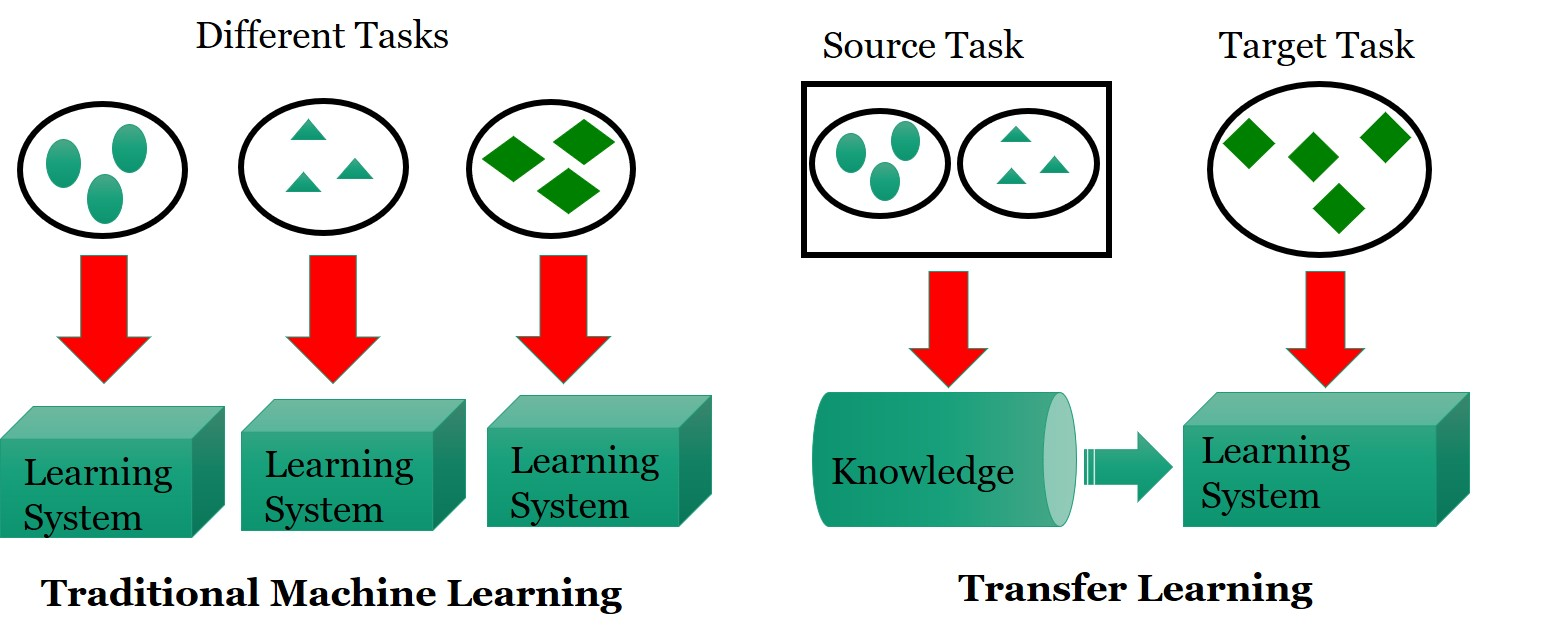
\includegraphics[width=4in,height=2in]{figures/TLGL}
%	\linebreak
%	\captionof{figure}{Conventional machine vs. transfer learning. Originally shown in~\cite{5288526}.}
%	\label{fig1:TLGL}
%\end{center}
%\end{figure}
\noindent
\enquote{What to transfer} sees which pieces of information can be transferred from one task or domain to another. Some information can be specific to a certain task or domain, and some information can be common across tasks or domains. After getting the information that can be transferred, different algorithms had been developed to deal with \enquote{how to transfer} the information. \enquote{When to transfer} figures out the criteria when transferring skills should be done. 
Transfer learning is categorized into three groups according to the labels availability in the source and target domains, and the tasks of the two domains. It is further discussed below.
\subsection{Inductive Transfer Learning}
In inductive transfer learning source and target tasks are different, and it does not matter source, and target domains are similar or different. In this case, labeled data in the target domain is required for induction. Based on the situation of labeled and unlabeled source domain, inductive transfer learning can further categorize in two cases.%\\

\noindent
\textbf{Multi-Task Learning.~}
In multi-task learning source and target tasks are learned simultaneously, it does not matter that the source and target domains are similar or different. The aim is to achieve high performance in the target task.%\\

\noindent
\textbf{Self-Taught Learning.~}
In self-taught-learning the source and target domains may have different label spaces, which show that we can not use directly side information of source domain.

\subsection{Transductive Transfer Learning}
The transductive transfer learning proposed by~\cite{arnold2007comparative}. For transductive transfer learning source and target tasks should be similar, but the domains can be different. Domain adaptation is a type of transductive transfer learning. In domain adaptation, source domain contains abundant labeled data while the target domain contains no labeled data, and the source and target domains are different. Different transductive transfer learning had been proposed. Structural Correspondence Learning (SCL) is one of them. The SCL was proposed for speech tagging. It uses the unlabeled target domain for reducing the domain data differences. Based on unlabeled data in both domains, the set of pivotal features are defined. These defined pivotal features are used to learn the mapping between original feature space and shared low-dimension feature space.
\subsection{Unsupervised Transfer Learning}
Unsupervised transfer learning is more focused to clustering, dimension reduction, where there is no need for labeled data in both source and target domains, while it is similar to multi-task learning where the source and target tasks are different but related to each other.\\

